\chapter{Objetivos}\label{cap.objetivos}
En este capitulo se presentan los propositos planteados para este proyecto y la metodología que se ha utilizado para alcanzarlos.

\section{Objetivos}
La principal meta de este trabajo es la de enriquecer con tecnologías web las herramientas robóticas existentes en la plataforma JdeRobot. Para alcanzar este objetivo, se ha dividido el trabajo en tres partes: 
\begin{enumerate}
\item Modificar los tres visores existentes elaboradas mediante tecnologías web en la plataforma JdeRobot (\texttt{CameraViewjs}, \texttt{KobukiViewerjs} y \texttt{UavViewerjs}) para su utilización con el middleware ROS, además de ICE como hasta ahora. 
\item Creación mediante tecnologías web de un nuevo visor que permitirá la visualización de elementos 3D (puntos, líneas y objetos 3D) usando WebGL.
\item Elaborar un nuevo driver robótico de imágenes utilizando tecnologías web y WebRTC, cuyo cometido será el de servir imágenes a los distintos visores existentes en JdeRobot.
\end{enumerate}
Además de desarrollar estas piezas software para su ejecución dentro del navegador, se utilizará el entorno web Electron en todos ellos para posibilitar que se puedan ejecutar como una aplicación de escritorio sobre diferentes sistemas operativos.

\section{Metodología}
La metodología elegida para la ejecución del trabajo ha sido el desarrollo en espiral. Se trata de uno de los modelos más utilizados en el desarrollo de software y consiste en la realización de una serie de ciclos o iteraciones que se repiten en forma de espiral.
\begin{figure}[H]
  \begin{center}
    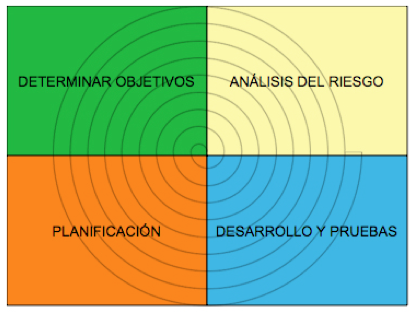
\includegraphics[width=0.8\textwidth]{figures/desarrolloespiral.png}
		\caption{Modelo de desarrollo en espiral}
		\label{fig.desarrolloespiral}
		\end{center}
\end{figure}
Cada iteración o ciclo está formado por cuatro etapas.
\begin{enumerate}
\item Determinación de los objetivos a alcanzar para que el ciclo sea finalizado de manera exitosa.
\item Analizar los riegos que conlleva las elecciones tomadas para realizar el desarrollo, y establecer alternativas para solventar los posibles inconvenientes.
\item Desarrollar y probar los objetivos establecidos en la primera fase.
\item Planificar las siguientes etapas del proyecto, teniendo en cuenta los resultados obtenidos en esta interacción.
\end{enumerate}
De cara a llevar un mejor del trabajo, se han tenido reuniones semanales con el tutor, en las que se marcaban los objetivos para la siguiente semana, se exponían dudas o posibles problemas  así como se establecen posibles alternativas, y se revisaba el trabajo previo. Con estas reuniones semanales se consigue tener flujo de trabajo constante y fluido, disminuyendo la posibilidad de quedar bloqueado en algún punto durante un largo periodo de tiempo.

Además, se ha elaborado un bitácora en la mediawiki\footnote{\url{https://jderobot.org/Rperez-tfg}} de JdeRobot, donde quede reflejado todos los progresos así como videos demostrativos de los avances. También se dispone de un repositorio en GitHub\footnote{\url{https://github.com/RoboticsURJC-students/2017-tfg-roberto-perez}} donde se ha ido subiendo todo el código para su verificación y prueba por terceras personas.

\section{Plan de Trabajo}
El plan de trabajo seguido es el siguiente:

\begin{enumerate}
\item Familiarización con las tecnologías robóticas que se van a utilizar en este trabajo: La plataforma JdeRobot, el simulador Gazebo y los middleware ICE y ROS
\item Entender el funcionamiento de las tecnologías web que se utilizarán en el desarrollo de las herramientas: El entorno Electron, WebGL, WebRTC y RobotWebTools para la compatibilidad de las tecnologías web con ROS.
\item Ampliación de las herramientas web existentes en la plataforma JdeRobot: Se adaptarán para ser usadas con Electron, y posteriormente se añadirá la compatibilidad con el middleware ROS, de modo que puedan ser usadas con ambos middleware de comunicación.
\item Creación de un nuevo visor de objetos 3D: Primero se revisará el visor utilizado hasta ahora y desarrollado con C++. Una vez conocido su funcionamiento, se creará el nuevo visor 3D adaptando las conexiones ICE del visor antiguo para que funcionen con el nuevo. Finalmente, se ampliará el visor para que pueda mostrar más primitivas además de los puntos que podía mostrar el antiguo, concretamente segmentos y modelos 3D de objetos cualesquiera.
\item Para terminar el trabajo, se implementará un nuevo driver que proporcionará un servidor de imágenes utilizando tecnologías web y WebRTC.
\end{enumerate}


